\documentclass{amsart}
\usepackage[utf8x]{inputenc}
\usepackage{pstricks,  amssymb}
\usepackage{tikz, tikz-cd}
\tikzcdset{scale cd/.style={every label/.append style={s}
      cells={nodes={scale=#1}}}}
\usetikzlibrary{arrows}
\usepackage{amsmath}

\newcommand{\NP}{\operatorname{Root}}

\newcommand{\Fl}{\operatorname{Fl}}

\newcommand{\F}{\mathcal{F}}

\newcommand{\NF}{\mathcal{N}}

\begin{document}

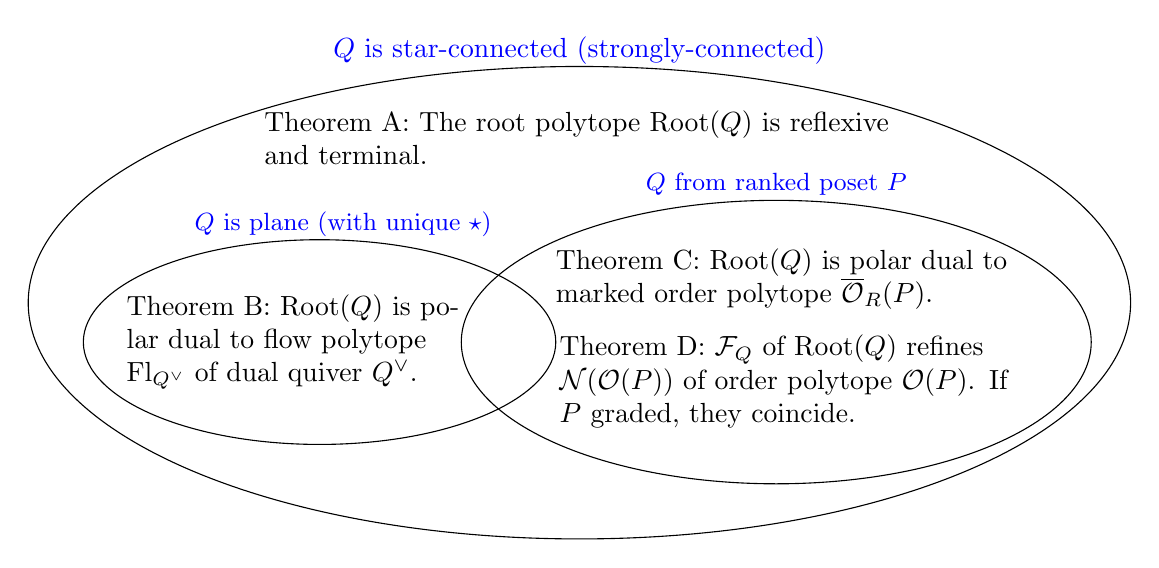
\begin{tikzpicture}
\draw (0,0) ellipse (7cm and 3cm);
    \draw (-3.3,-.5) ellipse(3cm and 1.3cm);
    \draw (2.5,-.5) ellipse(4cm and 1.8cm);
	\node
	at (0,3.2) {\blue{$Q$ is star-connected (strongly-connected)}};
	\node at (-3,1) {\blue{\small{$Q$ is plane (with unique $\star$)}}};
	\node at (2.5,1.5) {\blue{\small{$Q$ from ranked poset $P$}}};
	\node[text width=8cm] at (0,2.1) {Theorem A: The root %quiver Newton 
	polytope
	$\NP(Q)$ is reflexive and terminal.};
	\node[text width=4.5cm] at (-3.5,-0.5) {Theorem B: $\NP(Q)$ is 
	polar dual to flow 
	polytope $\Fl_{Q^\vee}$ of dual quiver 
	$Q^\vee$.};
	\node[text width=6cm] at (2.7,0.3) {Theorem C: $\NP(Q)$ is 
	polar dual to marked order polytope $\overline{\mathcal{O}}_R(P)$.};
	\node[text width=6.3cm] at (2.9,-1) {Theorem D: $\F_Q$ of 
	$\NP(Q)$ refines $\NF(\mathcal{O}(P))$ of order polytope $\mathcal{O}(P)$.  If $P$ graded, they coincide.};
\end{tikzpicture}

\end{document}